\section{Anhang A: Material, Zusatzdaten und erweiterte Nachweise}\label{sec:anhanga}

\subsection{Ergänzende Tabellen und Rohdaten}

\subsubsection{Datenbankschema (SQLite)}
Die folgenden SQL-Anweisungen beschreiben die Struktur der verwendeten Datenbank \texttt{database.db}. Die Tabellen bilden die Grundlage für das Berechtigungssystem.

\begin{lstlisting}[language=SQL]
CREATE TABLE IF NOT EXISTS cards (
  uid TEXT PRIMARY KEY,
  lastAssigned TEXT,
  isValid INTEGER
);

CREATE TABLE IF NOT EXISTS permissions (
  id INTEGER PRIMARY KEY AUTOINCREMENT,
  startDate TEXT,
  endDate TEXT,
  createdAt DATETIME DEFAULT CURRENT_TIMESTAMP,
  isRecurring INTEGER,
  recurrencePattern TEXT,
  isValid INTEGER,
  assignedStudent TEXT,
  assignedBy TEXT,
  FOREIGN KEY (assignedStudent) REFERENCES students(id),
  FOREIGN KEY (assignedBy) REFERENCES teachers(id)
);

CREATE TABLE IF NOT EXISTS students (
  id TEXT PRIMARY KEY,
  firstName TEXT,
  lastName TEXT,
  className TEXT,
  photoUrl TEXT,
  faceDescriptor TEXT,
  associatedCard TEXT,
  FOREIGN KEY (associatedCard) REFERENCES cards(uid)
);

CREATE TABLE IF NOT EXISTS teachers (
  id TEXT PRIMARY KEY,
  name TEXT,
  email TEXT,
  passwordHash TEXT,
  role TEXT DEFAULT 'teacher',
  permissions TEXT
);

CREATE TABLE IF NOT EXISTS accessLogs (
  id INTEGER PRIMARY KEY AUTOINCREMENT,
  kartenId TEXT,
  studentId TEXT,
  timestamp DATETIME DEFAULT CURRENT_TIMESTAMP,
  accessGranted INTEGER,
  verificationMethod TEXT,
  FOREIGN KEY (kartenId) REFERENCES cards(uid),
  FOREIGN KEY (studentId) REFERENCES students(id)
);
\end{lstlisting}

\subsubsection{API-Endpunkte}
In der folgenden Tabelle sind die wichtigsten API-Endpunkte des Backends aufgeführt, die von der Guard-App und dem Schüler-Interface genutzt werden.

\begin{longtable}{lll}
\caption{Übersicht der API-Endpunkte} \\
\toprule
\textbf{Methode} & \textbf{Pfad} & \textbf{Beschreibung} \\ \midrule
\endhead
POST & /auth/login & Authentifizierung für Personal \\
POST & /auth/login-student & Login für Schüler via ID \\
POST & /guard/validate & Validierung eines RFID-Scans \\
POST & /guard/verify-face & Vergleich von Snapshot und Referenz \\
GET & /student/profile & Abruf des Schülerprofils \\
POST & /cards/assign & Verknüpfung Karte mit Schüler \\ \bottomrule
\end{longtable}

\subsection{Ergänzende Abbildungen}
Die Benutzeroberfläche der Guard-App ist für die schnelle Verifikation optimiert. \autoref{fig:screenshot_guard} zeigt die Ansicht nach einem erfolgreichen RFID-Scan.

\begin{figure}[htbp]
  \centering
  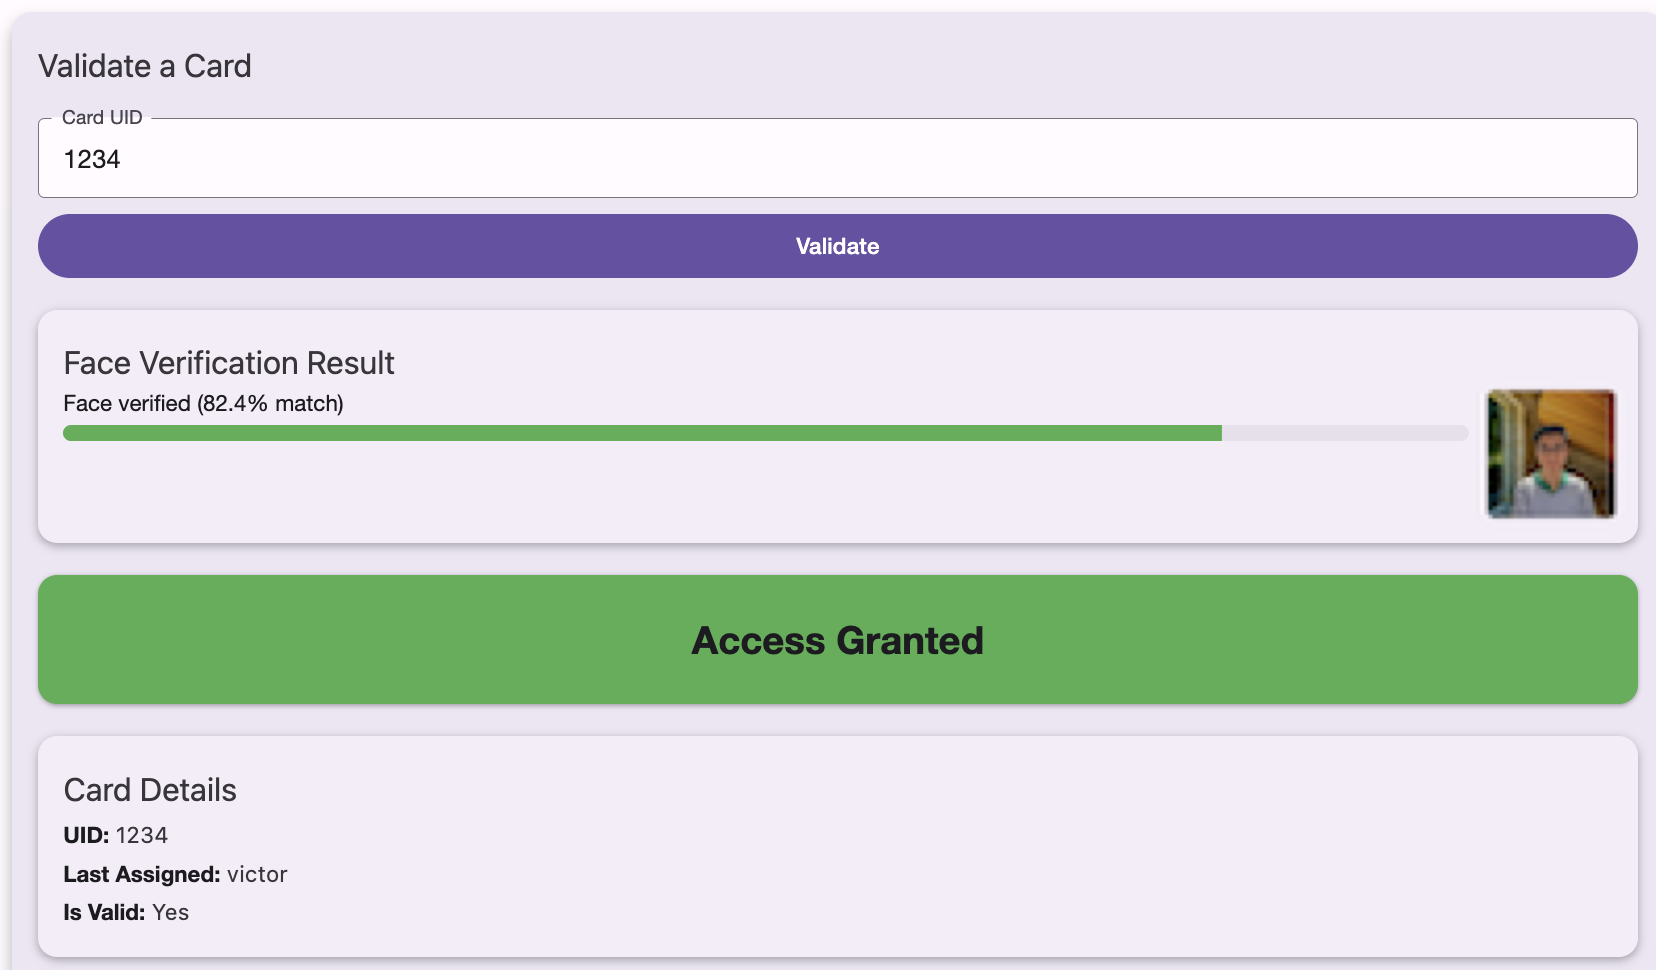
\includegraphics[width=0.8\textwidth,height=0.4\textheight,keepaspectratio]{figures/GuardAccessGranted.png}
  \caption{Benutzeroberfläche der Guard-App bei erfolgreicher Validierung}
  \label{fig:screenshot_guard}
\end{figure}

\subsection{Technische Artefakte}
Hier werden zentrale Code-Ausschnitte dokumentiert, die die technische Logik des Systems repräsentieren.

\subsubsection{Distanzberechnung (Euklidische Distanz)}
Die Entscheidung über eine Gesichtsübereinstimmung basiert auf der euklidischen Distanz der Face-Descriptoren.
\begin{lstlisting}
const distance = faceapi.euclideanDistance(
  snapshotDetection.descriptor,
  referenceDetection.descriptor
);
const threshold = 0.6;
const match = distance < threshold;
\end{lstlisting}

\subsubsection{HEIC-Konvertierungspipeline}
Die Normalisierung von iOS-Fotos erfolgt serverseitig durch eine Pipeline aus \texttt{heic-convert} und \texttt{sharp}.
\begin{lstlisting}
if (isHeicFormat || isHeifFormat) {
  heicBuffer = await heicConvert({
    buffer: imageBuffer,
    format: 'PNG',
    quality: 1
  });
  processedImageBuffer = Buffer.from(heicBuffer);
}
// Resize mit sharp auf Standardmass
const sharpOutput = await sharp(processedImageBuffer)
  .resize(1024, 1024, { fit: 'cover' })
  .png()
  .toBuffer();
\end{lstlisting}

\subsubsection{JWT-Authentifizierungs-Middleware}
Die Absicherung der Endpunkte erfolgt rollenbasiert mittels JSON Web Tokens.
\begin{lstlisting}
const checkAuth = (db, requiredPermissions = []) => {
  return (req, res, next) => {
    const token = req.headers.authorization.split(' ')[1];
    try {
      const decoded = jwt.verify(token, process.env.JWT_SECRET);
      req.user = decoded;
      if (requiredPermissions.length > 0) {
        const userPermissions = req.user.permissions || [];
        const hasPermission = requiredPermissions.every(p => userPermissions.includes(p));
        if (!hasPermission) return res.status(403).json({ error: 'Forbidden' });
      }
      next();
    } catch (err) {
      return res.status(401).json({ error: 'Unauthorized' });
    }
  };
};
\end{lstlisting}
